\chapter{Implementacija i korisničko sučelje}
		
		
		\section{Korištene tehnologije i alati}
		
			\textbf{\textit{dio 2. revizije}}
			
			 \noindent Za komunikaciju među članovima tima korišten je Whatsapp (https://www.whatsapp.com/), za raspodijelu zadataka među članovima tima korišten je Miro (https://miro.com/). Kao sustav za upravljanje izvornim kodom korišten je Git (https://git-scm.com/), a za udaljeni repozitorij projekta korišten je GitLab ( https://gitlab.com/). Za izradu UML dijagrama u dokumentaciji korišten je Astah UML (https://astah.net/).Za izradu backend dijela aplikacije korišten je programski jezik python (https://www.python.org/) verzija 3.8, te alat Flask (https://flask.palletsprojects.com/en/1.1.x/). Kao aplikacijski server korišten je heroku (https://heroku.com/).Korištena je baza podataka MySQL (https://www.mysql.com/).

			
			
			\eject 
		
	
		\section{Ispitivanje programskog rješenja}
			
			\textbf{\textit{dio 2. revizije}}\\
			
			 \textit{U ovom poglavlju je potrebno opisati provedbu ispitivanja implementiranih funkcionalnosti na razini komponenti i na razini cijelog sustava s prikazom odabranih ispitnih slučajeva. Studenti trebaju ispitati temeljnu funkcionalnost i rubne uvjete.}
	
			
			\subsection{Ispitivanje komponenti}
			
			\begin{figure}[H]
				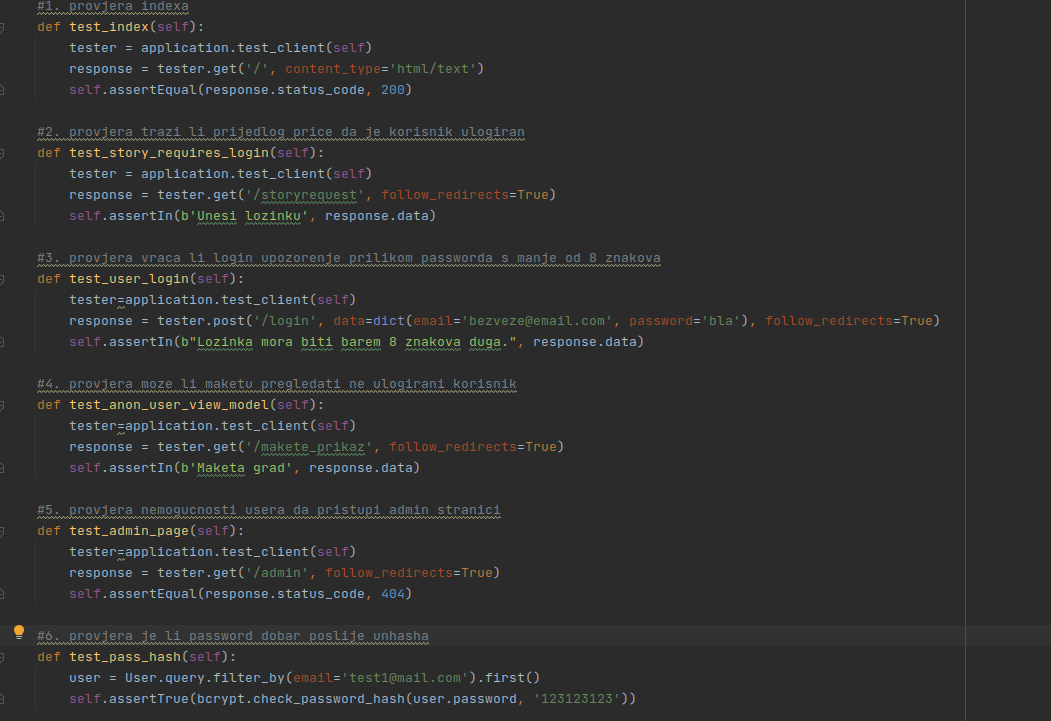
\includegraphics[width=1\linewidth]{slike/unit_tests.PNG} %veličina u odnosu na širinu linije
				\caption{Ispitivanje jedinica}
				\label{fig:unit1} %label mora biti drugaciji za svaku sliku
			\end{figure}
		
			\begin{figure}[H]
				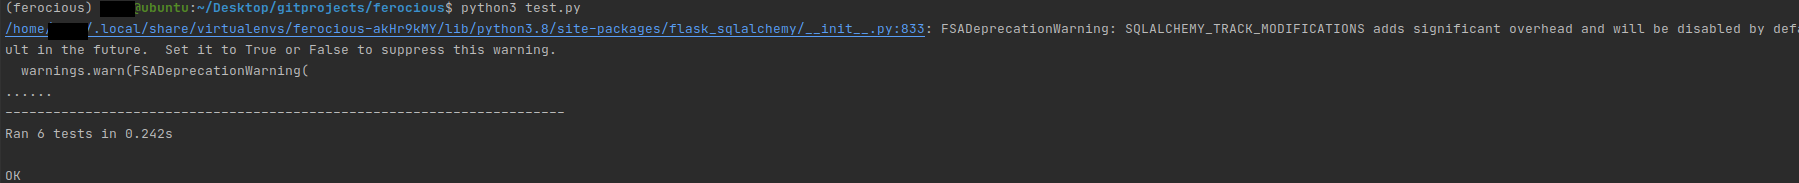
\includegraphics[width=1\linewidth]{slike/unit_test_result.PNG} %veličina u odnosu na širinu linije
				\caption{Rezultat ispitivanja jedinica}
				\label{fig:unit2} %label mora biti drugaciji za svaku sliku
			\end{figure}
			
			
			\subsection{Ispitivanje sustava}
			
			 \noindent Provedeno je testiranje rada sustava pomoću Selenium testova(Selenium IDE)
			 . Testirane su neke od osnovnih funkcionalnosti sustava. Svi testovi izvrseni su ručno. U dokumentaciji su prikazani slučajevi UC1, UC9, UC10, UC11, UC23.

			\noindent Ispitni slučaj 1 : Registracija

			\noindent Ulaz : 
	
			\begin{itemize}
				\item : 1. Otvaranje pocetne stranice u web pregledniku.
				\item   2. Odabir na gumb registracije
				\item   3. Unos potrebnih podataka
			\end{itemize}

			\noindent Ocekivani rezultat : 

			\begin{itemize}
				\item : 1.a Prikazao se ekran za unos podataka
				\item   1.b Ako su uneseni valjani podaci korisnik ce biti preusmjeren na login screen
			\end{itemize}
	
			\noindent Rezultati : Očekivani rezultat 1.b je zadovoljen. Aplikacija je prošla test. 

			\begin{figure}[H]
				\includegraphics[width=1\linewidth]{slike/ispitnit_test_1.PNG} %veličina u odnosu na širinu linije
				\caption{Ispitni test 1}
				\label{fig:Test1} %label mora biti drugaciji za svaku sliku
			\end{figure}
			
			\noindent Ispitni slučaj 2 : Prijava

			\noindent Ulaz : 
	
			\begin{itemize}
				\item : 1. Otvaranje pocetne stranice u web pregledniku.
				\item   2. Odabir na gumb prijava
				\item   3. Unos potrebnih podataka
			\end{itemize}

			\noindent Ocekivani rezultat : 

			\begin{itemize}
				\item : 1.a Prikazao se ekran za unos podataka
				\item   1.b Ako su uneseni valjani podaci korisnik ce biti preusmjeren na pocetnu stranicu
			\end{itemize}
	
			\noindent Rezultati : Očekivani rezultat 1.b je zadovoljen. Aplikacija je prošla test. 

			\begin{figure}[H]
				\includegraphics[width=1\linewidth]{slike/ispitnit_test_2.PNG} %veličina u odnosu na širinu linije
				\caption{Ispitni test 2}
				\label{fig:Test2} %label mora biti drugaciji za svaku sliku
			\end{figure}			

			\noindent Ispitni slučaj 3 : Odjava

			\noindent Ulaz : 
	
			\begin{itemize}
				\item : 1. Korisnik treba biti prijavljen
				\item   2. Odabir na gumb odjavi se
			\end{itemize}

			\noindent Ocekivani rezultat : 

			\begin{itemize}
				\item : 1. Korisnik će biti odjavljen i preusmjeren na pocetnu stranicu
			\end{itemize}
	
			\noindent Rezultati : Očekivani rezultat 1. je zadovoljen. Aplikacija je prošla test. 

			\begin{figure}[H]
				\includegraphics[width=1\linewidth]{slike/ispitnit_test_3.PNG} %veličina u odnosu na širinu linije
				\caption{Ispitni test 3}
				\label{fig:Test3} %label mora biti drugaciji za svaku sliku
			\end{figure}	

			\noindent Ispitni slučaj 4 : Odjava

			\noindent Ulaz : 
	
			\begin{itemize}
				\item : 1. Korisnik treba biti prijavljen
				\item   2. Odabir na gumb moj profil
			\end{itemize}

			\noindent Ocekivani rezultat : 

			\begin{itemize}
				\item : 1. Korisnik će biti preusmjeren na stranicu sa svojim podacima
			\end{itemize}
	
			\noindent Rezultati : Očekivani rezultat 1. je zadovoljen. Aplikacija je prošla test. 

			\begin{figure}[H]
				\includegraphics[width=1\linewidth]{slike/ispitnit_test_4.PNG} %veličina u odnosu na širinu linije
				\caption{Ispitni test 4}
				\label{fig:Test4} %label mora biti drugaciji za svaku sliku
			\end{figure}				

			\noindent Ispitni slučaj 5 : Postavljanje postavki vidljivosti korisničkog računa

			\noindent Ulaz : 
	
			\begin{itemize}
				\item : 1. Korisnik treba biti prijavljen
				\item   2. Odabir na gumb uredi
				\item   3. Odabir postavki vidljivosti
				\item   4. Pritisak na gumb spremi promjene
			\end{itemize}

			\noindent Ocekivani rezultat : 

			\begin{itemize}
				\item : 1.a Korisnik će biti preusmjeren na stranicu postavka profila
				\item   1.b Nakon odabira postavka privatnosti i pristika na gumb korisnik će biti preusmjeren na stranicu sa svojim podacima.
			\end{itemize}
	
			\noindent Rezultati : Očekivani rezultat 1.b je zadovoljen. Aplikacija je prošla test. 

			\begin{figure}[H]
				\includegraphics[width=1\linewidth]{slike/ispitnit_test_5.PNG} %veličina u odnosu na širinu linije
				\caption{Ispitni test 5}
				\label{fig:Test5} %label mora biti drugaciji za svaku sliku
			\end{figure}

			\eject 
		
		
		\section{Dijagram razmještaja}
			
			 Dijagram razmještaja je strukturni statički UML dijagram koji opisuje topologiju sustava i usredotočen je na odnos sklopovskih i programskih dijelova. Postoji više vrsta dijagrama razmještaja, a ovdje se koristi specifikacijski dijagram razmještaja kako bi se prije navedeni odnos prikazao. Za ostvarenje ove aplikacije se koristi arhitektura "klijent - poslužitelj", a komunikacija se odvija protokolom HTTP. Na klijentskoj strani se nalazi web preglednik pomoću kojeg korisnik pristupa poslužitelju, odnosno šalje HTTP zahtjeve i prima HTTP odgovore. Poslužiteljska strana je nešto složenija te se ona sastoji od web poslužitelja na koji pristižu HTTP zahtjevi i poslužitelja baze podataka kojem web poslužitelj pristupa i iz kojeg uzima, uređuje ili sprema podatke.
			 
			 \begin{figure}[H]
			 	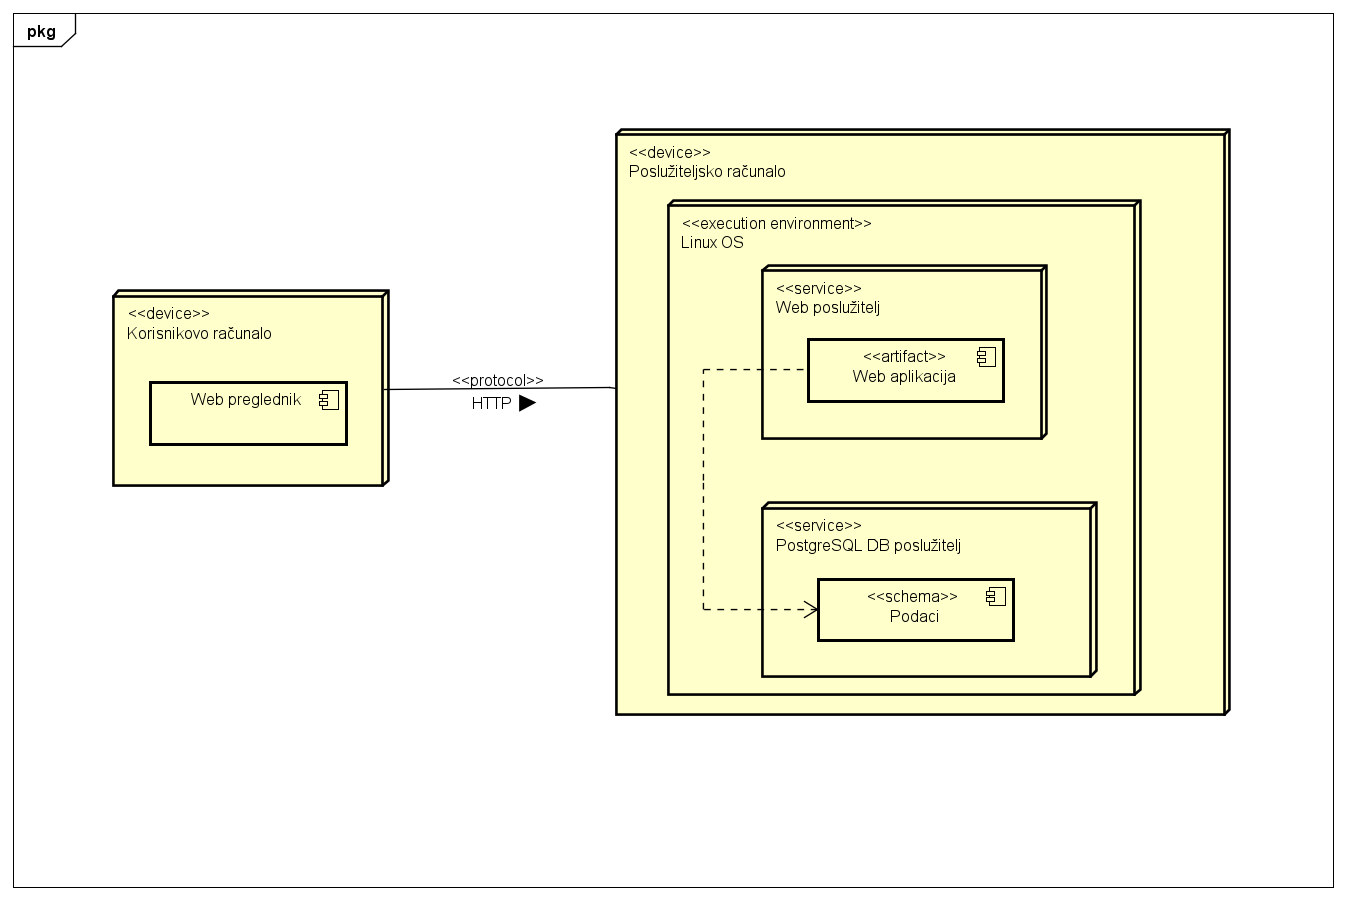
\includegraphics[width=1\linewidth]{slike/Dijagram_razmjestaja.PNG} %veličina u odnosu na širinu linije
			 	\caption{Dijagram razmještaja}
			 	\label{fig:dijraz} %label mora biti drugaciji za svaku sliku
			 \end{figure}
			
			\eject 
		
		\section{Upute za puštanje u pogon}
			\noindent\textbf{Heroku}\\
			Aplikacija je namjenjena puštanju u pogon preko platforme Heroku. Heroku je servis koji nudi usluge posluživanja aplikacija u više programskih jezika, među kojima su Ruby, Java, Node.js, Scala, Clojure, Python, PHP i Go, te usluge posluživanja baza podataka. Heroku je izabran za ovaj projekt zbog niske cijene (besplatan za stranicu ovog opsega) i jednostavnosti korištenja. Pretpostavit ćemo da korisnik na računalu ima instaliran Git te da je aplikacija preuzeta na računalo.
			\\\\
			\noindent\textbf{Stvaranje projekta}\\
			Potrebno je stvoriti račun na  \href{www.heroku.hr}{www.heroku.hr} te se prijaviti. Stranica će nas preusmjeriti na \textit{dashboard}, odakle stvaramo novi projekt klikom na gumb "New" - "Create new app" u gornjem desnom kutu grafičkog sučelja (Slika \ref{fig:newapp}). Pokazat će nam se forma za unos imena aplikacije i regije na kojoj će biti puštena u pogon (Slika \ref{fig:nameapp}). Nakon toga smo preusmjereni na stranicu novokreiranog projekta.
			\textbf{Napomena:} Ime aplikacije mora biti jedinstveno na razini čitave platforme. 
			\begin{figure}[H]
				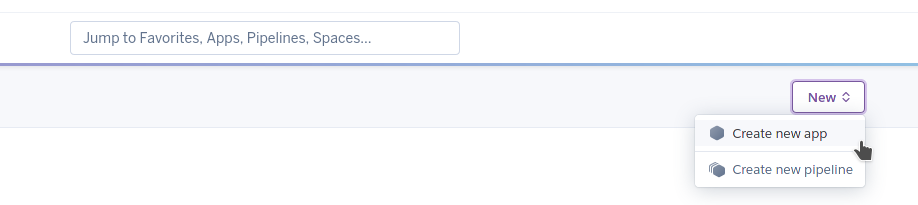
\includegraphics[width=.9\linewidth]{slike/20210114_203519.png}
				\centering
				\caption{Nova aplikacija}
				\label{fig:newapp}
			\end{figure}
			\begin{figure}[H]
				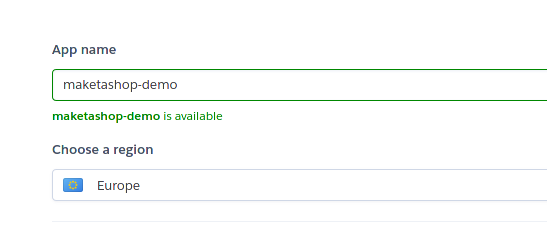
\includegraphics[width=.9\linewidth]{slike/20210114_203555.png}
				\centering
				\caption{Ime aplikacije}
				\label{fig:nameapp}
			\end{figure}
			\noindent\textbf{Stvaranje baze podataka}\\
			Heroku pruža uslugu posluživanje PostgreSQL baze podataka. Kako bismo ju omogućili, na stranici projekta kliknemo na "Resources" karticu (Slika \ref{fig:resourcestab}). U traci za pretraživanje poglavlja "Add-ons" upišemo pojam "Heroku Postgres" i odaberemo prvi rezultat (Slika \ref{fig:herokupostgres}). Odaberemo plan pri vrhu sučelja, te kliknemo "Submit Order Form" (Slika \ref{fig:orderform}).\\
			Sada navigiramo na "Settings"  karticu (Slika \ref{fig:settingstab}) i nađemo poglavlje "Config Vars". Kliknemo gumb "Reveal Config Vars" za prikaz varijabli okruženja te radimo dvije stvari. Prvo se uvjerimo da postoji varijabla "DATABASE\_URL" koja je nastala kada smo stvorili PostgreSQL bazu. Nakon toga u polje "KEY" upisujemo pojam "SECRET" \textit{(bez navodnika)} i u polje "VALUE" upisujemo bilo kakav niz znakova. On će služiti za enkripciju poruka koje aplikacija razmjenjuje. Unos potvrdimo klikom na gumb "Add". Sučelje bi trebalo izgledati slično slici \ref{fig:configvars)}.
			\begin{figure}[H]
				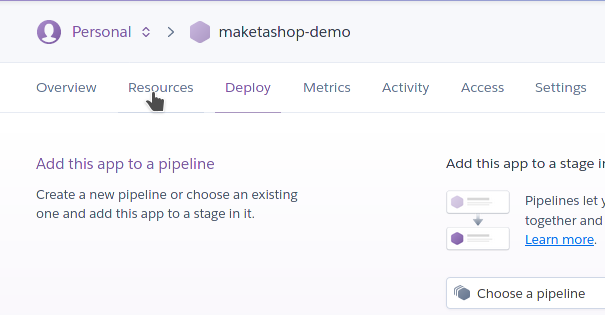
\includegraphics[width=.9\linewidth]{slike/20210114_214638.png}
				\centering
				\caption{Kartica "Resources"}
				\label{fig:resourcestab}
			\end{figure}
			\begin{figure}[H]
				
\includegraphics[width=.9\linewidth]{slike/20210114_215207.png}
				\centering
				\caption{Pretraživanje "Heroku Postgres"}
				\label{fig:herokupostgres}
			\end{figure}
			\begin{figure}[H]
				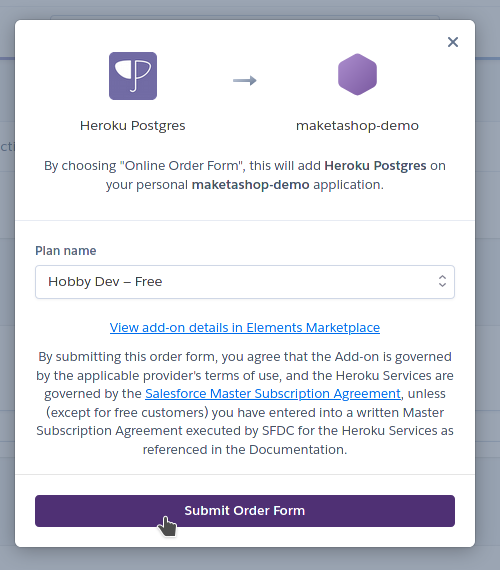
\includegraphics[width=.9\linewidth]{slike/20210114_214812.png}
				\centering
				\caption{"Submit Order Form"}
				\label{fig:orderform}
			\end{figure}
			\begin{figure}[H]
				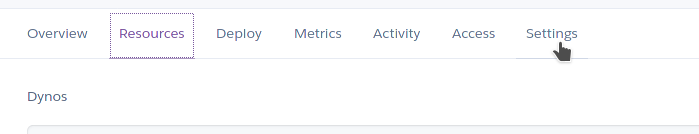
\includegraphics[width=.9\linewidth]{slike/20210114_215739.png}
				\centering
				\caption{"Settings" kartica}
				\label{fig:settingstab}
			\end{figure}
			\begin{figure}[H]
				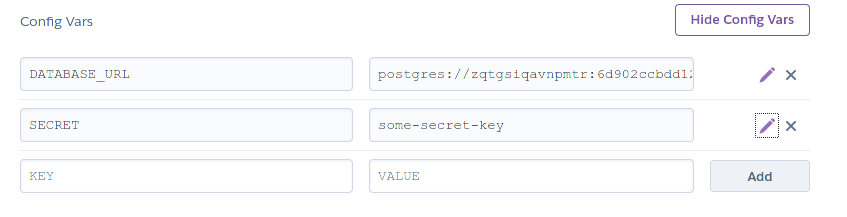
\includegraphics[width=.9\linewidth]{slike/20210114_220108.png}
				\centering
				\caption{Config Vars}
				\label{fig:configvars}
			\end{figure}
			\noindent\textbf{Heroku CLI}\\
			Heroku CLI \textit{(Command Line Interface)} nam omogućuje pristup platformi Heroku iz komandne linije. 
			Navigiramo nazad na karticu "Deploy". Kliknemo na poveznicu "Deployment method" - "Heroku Git" (Slika \ref{fig:herokucli)}) te pratimo uputstva za instalaciju ovisno o operacijskom sustavu koji koristimo.\\
			Po završetku instalacije otvorimo komandnu liniju \textit{cmd, terminal} i unesemo naredbu \code{heroku login}, nakon čega pratimo uputstva za prijavu.
			\begin{figure}[H]
				
\includegraphics[width=.9\linewidth]{slike/20210114_205522.png}
				\centering
				\caption{Heroku CLI}
				\label{fig:herokucli}
			\end{figure}
			\noindent\textbf{Spajanje Git repozitorija i Heroku}\\
			U komandnoj liniji se pozicioniramo na direktorij aplikacije \textit{(naredba cd)}. Za idući korak je bitno da imamo inicijaliziran Git repozitoriji u direktoriju. To možemo provjeriti naredbom \code{git status}. Ukoliko je ispis \code{fatal: not a git repository...}, inicijaliziramo ga naredbom \code{git init}. Nakon toga dodajemo Heroku udaljeni repozitoriji pomoću \code{heroku git:remote -a <ime-aplikacije>}, gdje \textit{ime-aplikacije} zamijenimo imenom koji smo odabrali pri kreaciji projekta.\\
			Sada \textit{pushamo} projekt na Heroku udaljeni repozitorij slijedećim nizom naredbi:\\
			\code{git add .}\\
			\code{git commit -am "Commit"}\\
			\code{git push heroku master}\\
			Ovo može potrajati oko 1 minute. Nakon toga Heroku preuzima stvar i puštanje u pogon se automatizira.
			\\\\
			\noindent\textbf{Pristup stranici}\\
			Vraćamo se na Heroku web-stranicu. Jedino što preostaje je u gornjem desnom kutu \textit{dashboarda} kliknuti na "Open App" što će nas preusmjeriti na aplikaciju (Slika \ref{fig:openapp}).
			\begin{figure}[H]
				
\includegraphics[width=.9\linewidth]{slike/20210114_222433.png}
				\centering
				\caption{Otvori aplikaciju}
				\label{fig:openapp}
			\end{figure}
			\eject 